\documentclass[a4paper,8pt]{article}
\pagestyle{plain}


\usepackage[utf8]{inputenc}
\usepackage{fancyhdr}
\usepackage[margin=2cm,foot=1cm]{geometry}
\usepackage[T1]{fontenc}
\usepackage{hyperref}
\usepackage{ragged2e}
\usepackage{pgf-umlcd}
\usepackage{graphicx,multicol}

\hypersetup{
	colorlinks,
	linkcolor={blue!80!black},
	citecolor={green!80!black},
	urlcolor={red!80!black}
}


% Used to set numbering of the content
\setcounter{tocdepth}{2}
\setcounter{secnumdepth}{3}

%%
% Math packages
\usepackage[utf8]{inputenc}
\usepackage{mathtools}
\usepackage{amssymb}
\usepackage{bm}
\usepackage{amsthm}
\usepackage{amsmath}
\usepackage{rotating}
\usepackage{mathrsfs}
\usepackage{tikz-cd}
\usepackage{float}
\usepackage{enumitem}

\graphicspath{ {./images/} }

%%
% Math Commands
\def\upint{\mathchoice%
	{\mkern13mu\overline{\vphantom{\intop}\mkern7mu}\mkern-20mu}%
	{\mkern7mu\overline{\vphantom{\intop}\mkern7mu}\mkern-14mu}%
	{\mkern7mu\overline{\vphantom{\intop}\mkern7mu}\mkern-14mu}%
	{\mkern7mu\overline{\vphantom{\intop}\mkern7mu}\mkern-14mu}%
	\int}
\def\lowint{\mkern3mu\underline{\vphantom{\intop}\mkern7mu}\mkern-10mu\int}
\usepackage{tikz}
\newcommand{\N}{\mathbb{N}}
\newcommand{\Lagr}{\mathcal{L}}
\newcommand{\R}{\mathbb{R}}
\newcommand{\Q}{\mathbb{Q}}
\newcommand{\C}{\mathbb{C}}
\newcommand{\x}{\mathbf{x}}
\newcommand{\F}{\mathbf{F}}
\newcommand{\f}{\mathbf{f}}
\newcommand{\y}{\mathbf{y}}
\renewcommand{\b}{\mathbf{b}}
\renewcommand{\c}{\mathbf{c}}
\renewcommand{\a}{\mathbf{a}}
\newcommand{\h}{\mathbf{h}}
\newcommand{\g}{\mathbf{g}}
\newcommand{\z}{\mathbf{z}}
\newcommand{\ze}{\mathbf{0}}
\newcommand{\Z}{\mathbb{Z}}
\newcommand{\norm}[1]{\left\lVert#1\right\rVert}
\newcommand{\abs}[1]{\left\lvert#1\right\rvert}
\newcommand{\brk}[1]{ \left[#1\right] }
\newcommand{\brc}[1]{ \left\{#1\right\} }
\newcommand{\paren}[1]{ \left(#1\right) }
\newcommand{\normop}[1]{\left\lVert#1\right\rVert_\text{op}}
\newcommand{\LL}{\mathcal{L}}
\newcommand{\uni}{\overset{\text{uni}}{\to}}
\DeclareMathOperator{\diam}{diam}
\newcommand{\Prr}[1]{\text{Pr}\left(#1\right)}
\newcommand{\code}[1]{\texttt{#1}}

\definecolor{dartmouthgreen}{rgb}{0.05, 0.5, 0.06}
\definecolor{egyptianblue}{rgb}{0.06, 0.2, 0.65}
\definecolor{dukeblue}{rgb}{0.0, 0.0, 0.61}
\definecolor{jazzberryjam}{rgb}{0.65, 0.04, 0.37}
\definecolor{magenta}{HTML}{EC008C}

%%
% Self-defined useful shortcuts
\newcommand{\isomorp}{\xrightarrow{\sim}}
\newcommand{\hlt}[1]{\textit{{\color{dukeblue}#1}}}
\newcommand{\impt}[1]{\textit{{\color{jazzberryjam}#1}}}
\newcommand{\qntype}[1]{\textit{{\color{dartmouthgreen}#1}}}
\newcommand{\soln}[1]{\textit{{\color{magenta}#1}}}
\newcommand{\gcds}[1]{\textnormal{gcd}#1}
\newcommand{\mins}[1]{\textnormal{min}#1}
\newcommand{\maxs}[1]{\textnormal{max}#1}
\newcommand{\lcms}[1]{\textnormal{lcm}#1}
\newcommand{\degs}[1]{\textnormal{deg}#1}
\newcommand{\exps}[1]{\textnormal{exp}#1}
\newcommand{\tors}[1]{\textnormal{Tor}#1}
\newcommand{\homs}[1]{\textnormal{Hom}#1}
\newcommand{\anns}[1]{\textnormal{Ann}#1}

%%
\setcounter{section}{0}
% Set up math tools
\theoremstyle{theorem}
\newtheorem{theorem}{Theorem}[section]
\newtheorem{corollary}[theorem]{Corollary}
\newtheorem{lemma}[theorem]{Lemma}
\newtheorem{proposition}[theorem]{Proposition}
\newtheorem{qnbank}[theorem]{Question Bank}
\let\oldqnbank\qnbank
\renewcommand{\qnbank}{\oldqnbank\normalfont}
\newtheorem{algorithm}[theorem]{Algorithm}
\let\oldalgorithm\algorithm
\renewcommand{\algorithm}{\oldalgorithm\normalfont}
\newtheorem{definition}[theorem]{Definition}
\let\olddefinition\definition
\renewcommand{\definition}{\olddefinition\normalfont}
\newtheorem{example}[theorem]{Example}
\let\oldexample\example
\renewcommand{\example}{\oldexample\normalfont}
\newtheorem{remark}[theorem]{Remark}
\let\oldremark\remark
\renewcommand{\remark}{\oldremark\normalfont}


\title{MA5251 Project 1}
\author{Li Xuanguang, A0154735B}

\begin{document}
\maketitle
\bibliographystyle{chicago}

\raggedright

\newpage

\tableofcontents

\newpage


\section{Conservation in the Equation}

First, we show that there is conservation. \newline

Given the equation
\begin{equation}
i \frac{\partial \psi(\bold{x}, t)}{\partial t} = -\frac{1}{2} \triangle_{\bold{x}} \psi(\bold{x}, t) + V(\bold{x}) \psi(\bold{x}, t) + \frac{1}{10} \abs{\psi(\bold{x}, t)}^2 \psi(\bold{x}, t) \nonumber
\end{equation}

We multiply this equation by the conjugate $\overline{\psi}$ and integrate with respect to $\bold{x}$
\begin{equation}
i \int \frac{\partial \psi}{\partial t} \overline{\psi} \ d \bold{x} = \frac{1}{2} \int \nabla\psi \cdot \overline{\nabla \psi} \ d \bold{x} + \int V \abs{\psi}^2 \ d \bold{x} + \frac{1}{10} \int \abs{\psi}^2 \abs{\psi}^2  \ d \bold{x} \nonumber
\end{equation}
Taking complex conjugate of entire equation, we then have
\begin{equation}
i \int \frac{\partial \overline{\psi}}{\partial t} \psi \ d \bold{x} = - \frac{1}{2} \int \overline{\nabla \psi} \cdot \nabla\psi \ d \bold{x} - \int V \abs{\psi}^2 \ d \bold{x} - \frac{1}{10} \int \abs{\psi}^2 \abs{\psi}^2  \ d \bold{x} \nonumber
\end{equation}

Adding both equations, we then have the following conservation result:
\begin{equation}
\frac{d}{dt} \int \abs{\psi(\bold{x}, t)}^2 \ d \bold{x} = 0 \nonumber
\end{equation}

\section{Spatial Semi-Discretisation}

We define the span as
\begin{equation}
X_N = \text{span}\left\{e^{ikx}e^{imy}e^{ipz} | \abs{k}, \abs{m}, \abs{p} \leq \frac{N}{2}\right\} \nonumber
\end{equation}

Hence, we can spatially discretise the function:
\begin{equation}
\psi_N(\bold{x}, t) = \sum\limits_{\bold{k} = \left\{-\frac{N}{2}, \ldots, \frac{N}{2} \right\}^3} \hat{\psi}_{\bold{k}} \text{exp}(i \bold{k} \cdot \bold{x}) = \sum\limits_{k = -\frac{N}{2}}^{\frac{N}{2}} \sum\limits_{m = -\frac{N}{2}}^{\frac{N}{2}} \sum\limits_{p = -\frac{N}{2}}^{\frac{N}{2}} \hat{\psi}_{k,m,p} (t) e^{ikx}e^{imy}e^{ipz} \nonumber
\end{equation}

Then we can use the Pseudo-spectral method
\begin{equation}
i \frac{\partial \psi_N}{\partial t} = -\frac{1}{2} \triangle_{\bold{x}} \psi_N + I_N (V \psi_N) + \frac{1}{10} \abs{\psi_N}^2 \psi_N \nonumber
\end{equation}

As a requirement of the Schrödinger equation, where
\begin{equation}
\frac{d}{dt} \int_{[0, 2\pi]^3} \abs{\psi_N (\bold{x}, t)}^2 \ d \bold{x} = 0 \nonumber
\end{equation}
referring to the lecture notes, we can approximate $V(\bold{x}) \psi_N(\bold{x}, t)$ by
\begin{align}
\tilde{F}(\bold{x}, t) &= \sum\limits_{\bold{k} = \left\{-\frac{N}{2}, \ldots, \frac{N}{2} \right\}^3} \tilde{F}_{\bold{k}}(t) \text{exp} (-i \bold{k} \cdot \bold{x}) \nonumber \\
\text{where \ \ \ \ } \tilde{F}_{\bold{k}} (t) &= \frac{1}{N^3} \sum\limits_{\bold{j} = \left\{0, \ldots, N-1 \right\}^3} V (\bold{x}_j) \psi_N (\bold{x}_j, t) \text{exp}(-i\bold{k} \cdot \bold{x}_{\bold{j}} ) \nonumber
\end{align}
Thus, we have the equation in form
\begin{equation}
\hat{\psi}^{'}_{\bold{k}} (t) = -i \frac{1}{2} \abs{\bold{k}}^2 \hat{\psi}_{\bold{k}} (t) - i \frac{1}{N^3} \sum\limits_{\bold{j} \in \{0, \ldots, N-1\}^3} \left[V(\bold{x}_{\bold{j}}) \psi_N(\bold{x}_{\bold{j}}, t) + \frac{1}{10} \abs{\psi_N(\bold{x}_{\bold{j}}, t)}^2 \psi_N(\bold{x}_{\bold{j}}, t) \right] \text{exp} (-i \bold{k} \cdot \bold{x}_{\bold{j}}) \nonumber
\end{equation}

Hence, we arrived at the following ODE:
\begin{align}
\hat{\psi}^{'}_{k,m,p} (t) &= -i \frac{1}{2}(k^2 + m^2 + p^2) \hat{\psi}_{k,m,p} (t) + \hat{f}_{k,m,p} (\hat{\bold{\psi}}), \nonumber \\
\hat{\bold{\psi}} &= \left(\hat{\bold{\psi}}_{-\frac{N}{2}, -\frac{N}{2}, -\frac{N}{2}}, \ldots,  \hat{\bold{\psi}}_{\frac{N}{2}, \frac{N}{2}, \frac{N}{2}} \right) \nonumber \\
\text{where \ \ \ } \hat{f}_{k,m,p} (\hat{\bold{\psi}}) &= -i \frac{1}{N^3} \sum\limits_{\bold{j} \in \{0, \ldots, N-1\}^3} \left[V(\bold{x}_{\bold{j}}) \psi_N(\bold{x}_{\bold{j}}, t) + \frac{1}{10} \abs{\psi_N(\bold{x}_{\bold{j}}, t)}^2 \psi_N(\bold{x}_{\bold{j}}, t) \right] \text{exp} (-i \bold{k} \cdot \bold{x}_{\bold{j}}) \nonumber
\end{align}

\section{Temporal-Discretisation}

Due to computational resource constraints, a first-order exponential Runge-Kutta Method is used.
\begin{equation}
\hat{\psi}^{n+1}_{k,m,p} = \text{exp}\left(-i\frac{1}{3}(k^2 + m^2 + p^2) \triangle t_n \right) \left(\hat{\psi}^{n}_{k,m,p} + \triangle t_n \hat{f}_{k,m,p} (\hat{\bold{\psi}}^n)\right) \nonumber
\end{equation}

\section{Computational Methodology}

Language: Python (V3.10) \newline

Python is used for clean code and version control, due to the ability to use Object Oriented Programming to control classes and functions. In addition, Python has several highly efficient packages, which was used for FFT computation. The package used is \code{scipy.fft.fftn} and \code{scipy.fft.ifftn}. The package \code{numpy} is used for matrix manipulation, and \code{matplotlib} for plotting. \newline

The class structure and function are as follows \newline

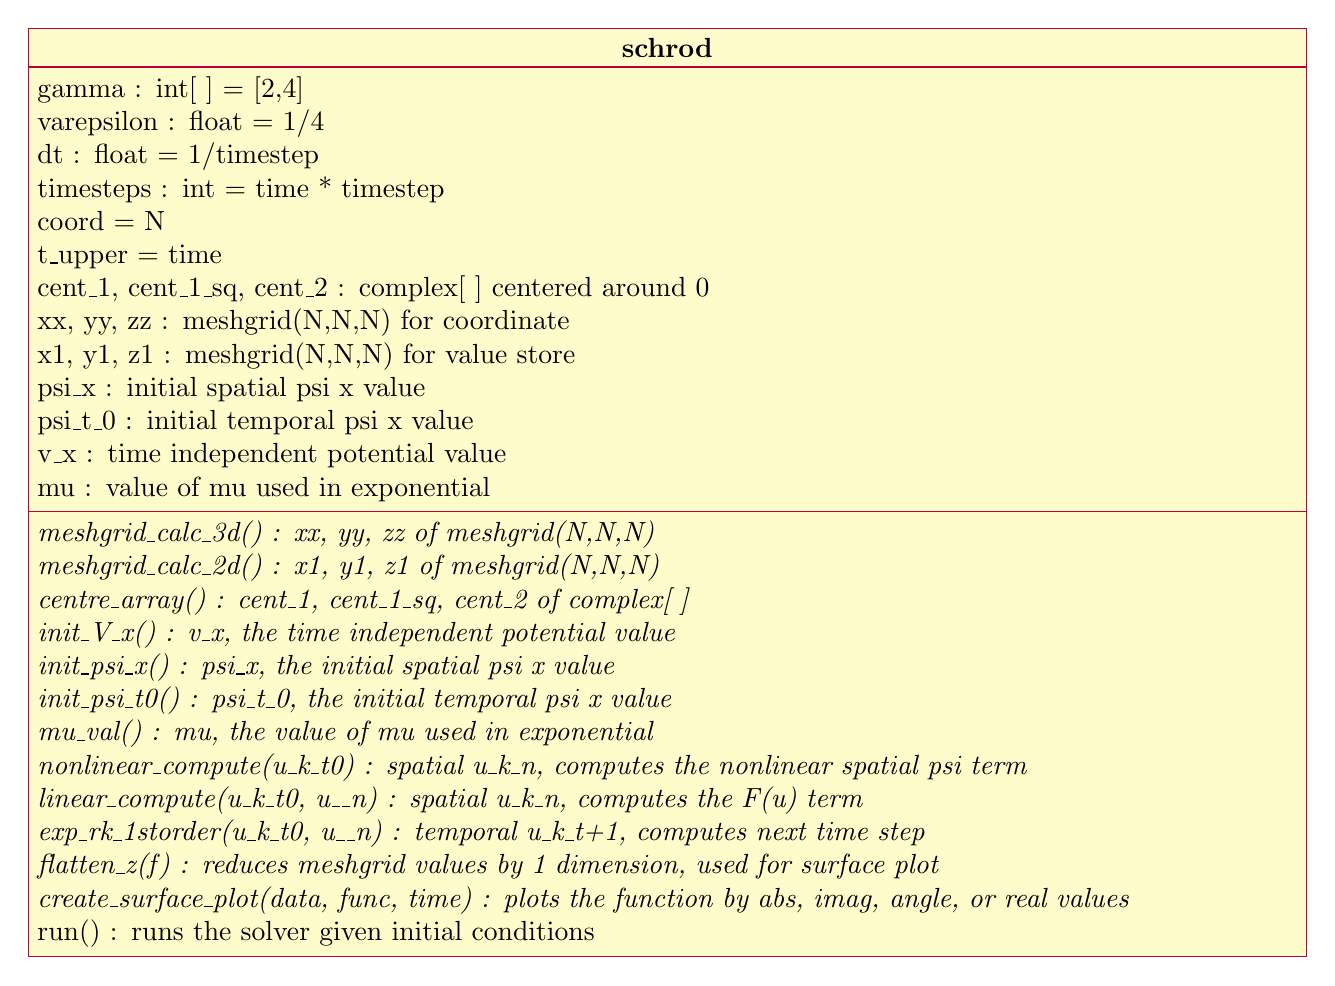
\begin{tikzpicture}
\begin{class}[text width=16cm]{schrod}{0,0}
\attribute{gamma : int[ ] = [2,4]}
\attribute{varepsilon : float = 1/4}
\attribute{dt : float = 1/timestep}
\attribute{timesteps : int = time * timestep}
\attribute{coord = N}
\attribute{t\_upper = time}
\attribute{cent\_1, cent\_1\_sq, cent\_2 : complex[ ] centered around 0}
\attribute{xx, yy, zz : meshgrid(N,N,N) for coordinate}
\attribute{x1, y1, z1 : meshgrid(N,N,N) for value store}
\attribute{psi\_x : initial spatial psi x value}
\attribute{psi\_t\_0 : initial temporal psi x value}
\attribute{v\_x : time independent potential value}
\attribute{mu : value of mu used in exponential}
\operation[0]{meshgrid\_calc\_3d() : xx, yy, zz of meshgrid(N,N,N)}
\operation[0]{meshgrid\_calc\_2d() : x1, y1, z1 of meshgrid(N,N,N)} 
\operation[0]{centre\_array() : cent\_1, cent\_1\_sq, cent\_2 of complex[ ]} 
\operation[0]{init\_V\_x() : v\_x, the time independent potential value} 
\operation[0]{init\_psi\_x() : psi\_x, the initial spatial psi x value} 
\operation[0]{init\_psi\_t0() : psi\_t\_0, the initial temporal psi x value} 
\operation[0]{mu\_val() : mu, the value of mu used in exponential} 
\operation[0]{nonlinear\_compute(u\_k\_t0) : spatial u\_k\_n, computes the nonlinear spatial psi term} 
\operation[0]{linear\_compute(u\_k\_t0, u\_\_n) : spatial u\_k\_n, computes the F(u) term} 
\operation[0]{exp\_rk\_1storder(u\_k\_t0, u\_\_n) : temporal u\_k\_t+1, computes next time step} 
\operation[0]{flatten\_z(f) : reduces meshgrid values by 1 dimension, used for surface plot} 
\operation[0]{create\_surface\_plot(data, func, time) : plots the function by abs, imag, angle, or real values} 
\operation{run() : runs the solver given initial conditions} 
\end{class}
\end{tikzpicture}\newline

Run the code in Python directly with command \code{python LI\_XUANGUANG\_A0154735B\_PRJ1.py}.\newline

The computational steps are as follows:
\begin{enumerate}[label=\arabic*.]
\setlength{\itemsep}{0pt}
\item Initialise the $V(x)$, $\psi(x, 0)$ variables
\item For $i$ in \code{range(0, timesteps)}, compute the inputs for the next time step by
\begin{enumerate}[label=\roman*.]
\setlength{\itemsep}{0pt}
\item Compute the Fourier transform of $\psi(x,t)$ to get $\psi(t)$
\item \code{scrhod.nonlinear\_compute} to compute nonlinear term
\item \code{scrhod.linear\_compute} to compute overall $F(u)$ term
\item \code{scrhod.exp\_rk\_1storder} to compute the next time step $\psi(x,t+1)$
\end{enumerate}
\end{enumerate}

\newpage

\section{Numerical Results and Discussion}

As the program is very computationally heavy and time consuming, a lower number of $N$ and a higher timestep $\triangle t$ is used. The parameters used are as follows:
\begin{enumerate}[label=\arabic*.]
\setlength{\itemsep}{0pt}
\item \code{N = 20}
\item \code{$\triangle$t = 0.01}
\item \code{t\_upper = 40} for $t=5k$, $k = 0, 1, \ldots, 8$
\end{enumerate}

As seen from the figures, the peaks gradually decrease and the wave function spreads fast, before resulting in a very low absolute value. The plots are submitted as part of the submission package.

\begin{figure}[h!]
\begin{multicols}{2}
\centering
\includegraphics[width=1\linewidth]{t0real}\\
Real value surface graph, $t=0$
\includegraphics[width=1\linewidth]{t5real}\\
Real value surface graph, $t=5$
\includegraphics[width=1\linewidth]{t10real}\\
Real value surface graph, $t=10$
\includegraphics[width=1\linewidth]{t0real3d}\\
Real value 3D graph, $t=0$
\includegraphics[width=1\linewidth]{t5real3d}\\
Real value 3D graph, $t=5$
\includegraphics[width=1\linewidth]{t10real3d}\\
Real value 3D graph, $t=10$
\end{multicols}
\end{figure}

\newpage

\begin{figure}[h!]
\begin{multicols}{2}
\centering
\includegraphics[width=1\linewidth]{t15real}\\
Real value surface graph, $t=15$
\includegraphics[width=1\linewidth]{t20real}\\
Real value surface graph, $t=20$
\includegraphics[width=1\linewidth]{t25real}\\
Real value surface graph, $t=25$
\includegraphics[width=1\linewidth]{t15real3d}\\
Real value 3D graph, $t=15$
\includegraphics[width=1\linewidth]{t20real3d}\\
Real value 3D graph, $t=20$
\includegraphics[width=1\linewidth]{t25real3d}\\
Real value 3D graph, $t=25$
\end{multicols}
\end{figure}

\newpage

\begin{figure}[h!]
\begin{multicols}{2}
\centering
\includegraphics[width=1\linewidth]{t30real}\\
Real value surface graph, $t=30$
\includegraphics[width=1\linewidth]{t35real}\\
Real value surface graph, $t=35$
\includegraphics[width=1\linewidth]{t40real}\\
Real value surface graph, $t=40$
\includegraphics[width=1\linewidth]{t30real3d}\\
Real value 3D graph, $t=30$
\includegraphics[width=1\linewidth]{t35real3d}\\
Real value 3D graph, $t=35$
\includegraphics[width=1\linewidth]{t40real3d}\\
Real value 3D graph, $t=40$
\end{multicols}
\end{figure}

\section{Disclosure}

This project has been done in discussion with another classmate, Song Zhigao.

%{\color{white}space}
%\begin{enumerate}[label=\roman*.]
%\setlength{\itemsep}{0pt}
%\item
%\end{enumerate}

%\begin{itemize}
%\setlength{\itemsep}{0pt}
%\item 	
%\end{itemize}

%\raggedright

%\begin{figure}[H]
%\centering
%\includegraphics[scale=0.4]{dihedralgroups}
%\caption{Example of an equilateral triangle as a Dihedral Group $D_6$}
%\end{figure}


\end{document}
